% =============================================================================
% HIKET -- INTERNAL PROGRESS TALK, October 2026.
%
% WHAT THIS IS. A ~20-minute talk that walks the storyline of the manuscript
% draft (manuscript/HIKET_draft_v1.tex, 2026-09-11 state) in the order the paper
% tells it: the soil that is still catching up -> the steady-state convention and
% what it cannot do -> the design (six models, transient start, equal information)
% -> the three results -> conclusions. Backup slides after \appendix for questions.
%
% FIGURES ARE NOT COPIED. Every \includegraphics resolves through \graphicspath to
% manuscript/figures/ (and the NextGenC thumbnails), so the deck follows the figure
% pipeline: rebuild a figure there and the slide updates on the next compile.
% Numbers quoted in the text are from production run 20260831_1624* (arm B),
% i.e. the same run the draft quotes.
%
% BUILD.  cd Reporting/October2026_internal_report && pdflatex HIKET_October2026_internal.tex
%         (twice for the slide counter). pdflatex is enough; metropolis falls back to
%         standard fonts. Speaker notes are in \note{} blocks -- switch the
%         \setbeameroption line below to show them.
%
% TIMING BUDGET (main part, 20 slides incl. title): ~1 min per slide, a little
% more on the four result figures (F3 mean SOC, F9, F14, F15), less on the text slides.
% Weight budget of the paper, deliberately mirrored: ~55% national trend,
% ~25% ridge position, ~20% plot-scale variance.
% =============================================================================
\documentclass[aspectratio=169,11pt]{beamer}
\usetheme[numbering=fraction,progressbar=frametitle,block=fill,sectionpage=none]{metropolis}
\usepackage[utf8]{inputenc}\usepackage[T1]{fontenc}
\usepackage{graphicx}\usepackage{booktabs}\usepackage{amsmath}
\usepackage{tikz}
\setbeameroption{hide notes}          % {show notes on second screen=right} to rehearse
\graphicspath{{../../manuscript/figures/}{../NextgenC_report/SOC_maps/thumbnails/}{../NextgenC_report/}}

% --- palette: keep close to the per-model colours used in the figures ---------
\definecolor{hiketDark}{RGB}{35,55,59}
\definecolor{hiketAccent}{RGB}{204,85,0}
\definecolor{hiketGreen}{RGB}{30,120,90}
\setbeamercolor{progress bar}{fg=hiketAccent}
\setbeamercolor{title separator}{fg=hiketAccent}
\setbeamercolor{frametitle}{bg=hiketDark}
\setbeamercolor{alerted text}{fg=hiketAccent}

% one-line takeaway at the bottom of a figure slide
\newcommand{\takeaway}[1]{\vspace{-0.3em}\begin{center}\footnotesize\textbf{#1}\end{center}}
% a figure filling the slide with the takeaway underneath
\newcommand{\figslide}[3]{% #1 file  #2 height (fraction of textheight)  #3 takeaway
  \vspace{-0.5em}
  {\centering\includegraphics[height=#2\textheight,width=\textwidth,keepaspectratio]{#1}\par}
  \vspace{0.15em}
  {\footnotesize\bfseries #3\par}}
\setbeamerfont{title}{size=\large}
\setbeamerfont{subtitle}{size=\small}

\title{Relaxing the steady-state assumption displaces forest soil carbon models along the trade-off between litter input and turnover}
\subtitle{HIKET --- internal progress talk: where the manuscript stands}
\author{Lorenzo Menichetti \\ \small with Aleksi Lehtonen, Samuli Launiainen, Boris Tupek, Olli-Pekka Tikkasalo}
\date{October 2026}

\begin{document}

\maketitle

% =============================================================================
% OPENING -- the soil that is still catching up
% =============================================================================
\section{The question}

\begin{frame}{Finnish forest soils have been measured three times}
  \figslide{F3_mean_SOCalt}{0.72}{The stock rose by $+0.259 \pm 0.040$ tC\,ha$^{-1}$\,yr$^{-1}$ over the whole window, but only $+0.117 \pm 0.066$ over the last interval. The accumulation is slowing down.}
  \note{Balanced set, n = 310, plots measured in all three campaigns. 64.5 -> 71.5 -> 73.6 tC/ha. First campaign drawn at its mean sampling year (~1989), because its fieldwork ran 1986-1995. The full-window rate is the robust one (survives a 9\% shared campaign offset); the last-interval rate is the fragile one (2\% removes it). The paper's opening claim rests partly on the fragile one; the model comparison rests on the robust one.}
\end{frame}

\begin{frame}{Why the trajectory, and not the stock, is the quantity that matters}
  \small
  \begin{columns}[T]
    \begin{column}{0.52\textwidth}
      \begin{itemize}
        \item A national inventory reports the \alert{annual change} of the soil stock, not the stock.
        \item In Finland the soil term is \alert{modelled}: NFI $\to$ litter $\to$ Yasso07 $\to$ $\Delta$SOC. No soil measurement enters the chain.
        \item Forest-land mineral soils, 2022: sink of \alert{4.8 Mt CO$_2$} against a biomass sink of 12.6 Mt; reported uncertainty \alert{31.5\%} vs 16.3\%.
        \item The land-use sector is already a net source ($+4.4$ Mt CO$_2$e). A term of that size and uncertainty decides the sign.
      \end{itemize}
    \end{column}
    \begin{column}{0.46\textwidth}
      \begin{block}{The awkward step}
        A model has to be told how much C the soil holds on day one, and how it is split between pools --- for a soil whose history was never observed.
      \end{block}
      \vspace{0.5em}
      \small Sweden measures its soil term by resampling its NFI plots (NID 2026). Most countries cannot afford that, and model it instead.
    \end{column}
  \end{columns}
  \note{Careful: ROMULv is NOT in the inventory -- Yasso07 alone. Lehtonen et al. 2016 is an evaluation. "Often modelled rather than measured" -- Sweden is the counterexample.}
\end{frame}

\begin{frame}{The convention: start the soil in balance with its litter input}
  \small
  \begin{columns}[T]
    \begin{column}{0.5\textwidth}
      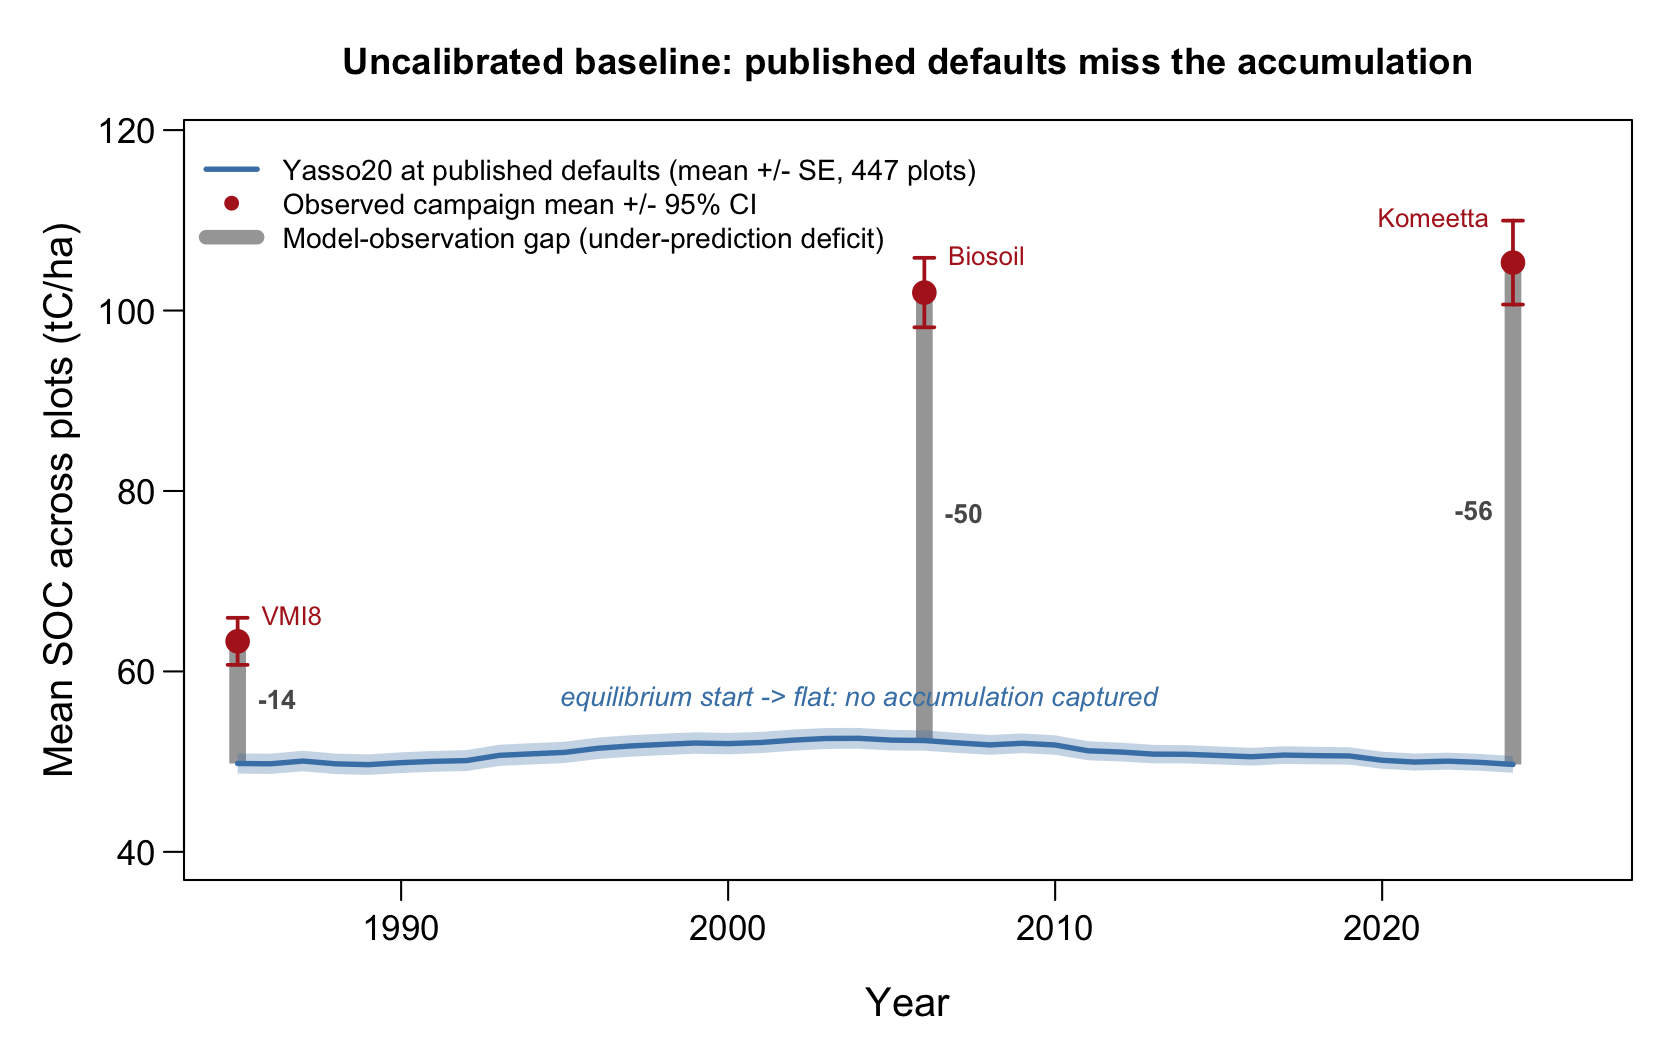
\includegraphics[width=\textwidth,height=0.46\textheight,keepaspectratio]{F2_baseline}
      \vspace{-0.6em}
      {\scriptsize Yasso20, published parameters, steady-state start: flat and low.}
    \end{column}
    \begin{column}{0.5\textwidth}
      \begin{itemize}
        \item Shared across lineages: Yasso, RothC, Century, global land-model spin-ups; CBM-CFS3 cycles to a repeating average.
        \item The Finnish inventory spins up on NFI6 litter (1971--76) and 1960--90 climate; its defence is Peltoniemi et al.\ 2006 --- a \alert{precision} study around an assumed level (``precision, not accuracy'').
        \item Liski et al.\ 2006 is our direct antecedent: same country, model family and NFI litter --- and they \emph{assumed} the 1922 state, having no repeated soil measurement.
      \end{itemize}
    \end{column}
  \end{columns}
  \takeaway{A soil started in balance has no accumulation left to perform.}
  \note{Frame Liski 2006 as lineage, not correction (Aleksi, Mikko are coauthors). Frame Peltoniemi 2006 as scope. Wutzler & Reichstein 2007 already criticised equilibrium fitting with Yasso -- we are not the first.}
\end{frame}

\begin{frame}{Finland is the wrong place for that assumption}
  \figslide{F10b_forest_history}{0.64}{Growing stock $+84\%$ over a century, most of it after the late 1960s. Litter follows biomass, so the input the models must integrate has been rising the whole time --- and unmanaged stands hold $\sim$40\% more mineral-soil C (Kumpu et al.\ 2025).}
  \note{Early 20th century: slash-and-burn, forest grazing, tar burning, selective removal -- historical low of standing volume. Peltoniemi 2004: trend cannot be distinguished unless measurements cover two rotations. Now we have three campaigns over ~4 decades.}
\end{frame}

\begin{frame}{Three questions, weighted in this order}
  \begin{enumerate}
    \item[\textbf{Q1}] Does a \alert{transient, calibrated initial state} reproduce the observed national SOC trajectory --- and what does reproducing it \emph{require} of the models? {\small (weight $\sim$55\%)}
    \item[\textbf{Q2}] Does it matter, for projection, \alert{where a calibration lands} on the exchange between litter input and transit time? {\small (weight $\sim$25\%)}
    \item[\textbf{Q3}] What part of the variation between \alert{individual plots} can none of the models see? {\small (weight $\sim$20\%)}
  \end{enumerate}
  \vspace{1em}
  \begin{block}{Two quantities govern a stock}
    litter input $J$ and mean transit time $\tau$: at balance $C^{*} = J\,\tau$. A stock fixes the product only. A trajectory can do more.
  \end{block}
\end{frame}

% =============================================================================
% ACTION -- the design
% =============================================================================
\section{The design}

\begin{frame}{Six models, two roles, one frame}
  \footnotesize
  \begin{columns}[T]
    \begin{column}{0.5\textwidth}
      \small
      \scriptsize
      \begin{tabular}{lccl}
        \toprule
        Model & Pools & Free & Role \\
        \midrule
        SP1 & 1 & 6 & benchmark \\
        TP2 & 2 & 7 & benchmark \\
        TP3 & 3 & 9 & benchmark \\
        Yasso07 & 5 & 20 & \textbf{the inventory model} \\
        Yasso15 & 5 & 26 & successor \\
        Yasso20 & 5 & 26 & successor \\
        \bottomrule
      \end{tabular}
      \vspace{0.4em}

      \footnotesize The simple models are a transparent ladder: any Yasso result is checked against a structure one can follow by hand.
    \end{column}
    \begin{column}{0.5\textwidth}
      \begin{block}{Equal \emph{external information}, not equal DoF}
        \begin{itemize}
          \item Yasso: rates \textbf{fixed} at published values; the 12 transfer fractions, climate, woody size are free.
          \item SP1/TP2/TP3: rates \textbf{anchored on ICBM} (fast fixed, slow pinned by a tight prior); humification fractions free.
          \item Priors homogenised in \emph{construction}, not in value: same rule per parameter class, centre from each model's own publication.
          \item All six integrate the linear system exactly; no explicit Euler step.
        \end{itemize}
      \end{block}
    \end{column}
  \end{columns}
  \note{Why rates fixed: a rate defines the pool -- changing it redefines the pool. Fractions are what the published Yasso calibrations themselves estimate. Why the simple models are pinned rather than fixed: ICBM rates come from an arable experiment; the slow-rate posterior width is a transferability diagnostic.}
\end{frame}

\begin{frame}{The move: estimate the starting state instead of assuming it}
  \figslide{F4_initialization}{0.66}{Start in 1917 in balance with the 1917 litter; raise the input along the Liski et al.\ 2006 reconstructed shape to 1985; then drive with the annual record. Two auxiliary parameters: $\sigma_{\mathrm{init}} = J_{1917}/J_{1985}$ and $\sigma_{\mathrm{input}}$, a multiplier on the whole litter series.}
  \note{The shape is taken from a reconstructed INPUT, not the growing stock: standing volume is a stock and misses harvest residues; the reconstructed input peaks around 1960. Only the shape is used, rescaled 0->1; the endpoints are the estimated quantities. Uncertainty of both sigmas propagates into the initial state AND the forward trajectory.}
\end{frame}

\begin{frame}{Data and error model, in one slide}
  \footnotesize
  \begin{columns}[T]
    \begin{column}{0.5\textwidth}
      \textbf{Observations}
      \begin{itemize}
        \item 456 NFI plots, 1205 plot-years; 365 fitted / 91 held out (by plot).
        \item Three campaigns rebuilt on \alert{one basis}: bulk density, coarse fragments (median 43\%, a $1.6\times$ effect), per-plot depth, modelled deep tail (validated on held-out 40--80 cm).
                \item Official 2006/2024 national stocks reproduced to 0.01 t/ha. First campaign: 2006 litter+moss layer added; \alert{true sampling year} used.
      \end{itemize}
    \end{column}
    \begin{column}{0.5\textwidth}
      \textbf{Litter and climate}
      \begin{itemize}
        \item Tupek et al.\ tree-litter product, AWEN $\times$ size class; $\bar J = 2.511$ tC\,ha$^{-1}$\,yr$^{-1}$; understorey \emph{not} included by design.
        \item FMI 10 km daily grid; climate modifier computed per year, then averaged (Jensen).
      \end{itemize}
      \textbf{Likelihood}
      \[
        \log y_{ij} = \log f_{ij}(\theta) + u^{R}_{r(i)} + u^{P}_{i} + u^{C}_{j} + e_{ij}
      \]
      \small Total SD fixed at 0.800, split (never added): region 0.117, plot 0.396, campaign 0.06/0.03, residual 0.685. Offsets marginalised; $\Sigma$ constant $\Rightarrow$ one triangular solve per evaluation.
    \end{column}
  \end{columns}
  \note{Why 0.800 above the measured 0.71-0.74: treating plot-years as independent understates what observations share (ICC 0.57-0.71; regional SE x2.3). DEzs, 5 runs x 50000, 15 chains. All R-hat <= 1.008, ESS >= 1450.}
\end{frame}

% =============================================================================
% RESOLUTION -- Q1
% =============================================================================
\section{Result 1 --- the national trajectory}

\begin{frame}{All six models reach the observed stocks}
  \figslide{F3_mean_soc}{0.66}{No model sits more than 3.5 tC/ha from any campaign mean --- with anchored rates, a constrained input and an estimated start. A precondition, not a result: any $J \times \tau$ with the same product reaches the same stock.}
  \note{Reaching the stock is NOT free here: rates are anchored, sigma_input has a 0.25 log-SD prior around an externally derived centre, the start is estimated. That all six get there is evidence that the frame is fair. The SHAPES differ: 07/15 rise and flatten; TP2/TP3 keep rising; SP1/Yasso20 peak late 2000s and decline.}
\end{frame}

\begin{frame}{\ldots and bracket the observed rate of change}
  \figslide{F5_stock_change}{0.66}{Observed $+0.259$; Yasso07 $+0.258$, Yasso15 $+0.250$; TP2/TP3 stronger, SP1/Yasso20 weaker. The bracketing is the result. Which model lands closest is \emph{not} interpretable --- reported as consistency, never validation.}
  \note{Three reasons the ranking is not interpretable: models not selected for it; observed rate has its own campaign-comparability uncertainty; between-model spread is a diagnostic, not an uncertainty estimate. The shape (accumulation that slows) is what a steady-state start discards -- reproducing it is the first result.}
\end{frame}

\begin{frame}{Model structure is nearly invisible in the fit}
  \footnotesize
  \begin{columns}[T]
    \begin{column}{0.58\textwidth}
      \scriptsize
      \begin{tabular}{lcccccc}
        \toprule
        Model & Pools & Free & $R^2$ cal & $R^2$ hold & RMSE & Eff.\ flux \\
        \midrule
        SP1     & 1 & 6  & 0.017 & 0.000 & 47 & 3.2 \\
        TP2     & 2 & 7  & 0.016 & 0.000 & 48 & 4.3 \\
        TP3     & 3 & 9  & 0.015 & 0.000 & 49 & 4.3 \\
        Yasso07 & 5 & 20 & 0.019 & 0.000 & 48 & 4.0 \\
        Yasso15 & 5 & 26 & 0.021 & 0.001 & 47 & 3.9 \\
        Yasso20 & 5 & 26 & 0.016 & 0.000 & 47 & 4.2 \\
        \bottomrule
      \end{tabular}
      \vspace{0.4em}

      {\tiny Table 1 of the draft. Effective flux $=\sigma_{\mathrm{input}}\,\bar J$, tC\,ha$^{-1}$\,yr$^{-1}$; RMSE on held-out plots, tC/ha.}
    \end{column}
    \begin{column}{0.42\textwidth}
      \begin{itemize}
        \item Held-out $R^2$ is zero to three decimals in all six; RMSE spans 3.6\% best to worst.
        \item Skill does not climb the pool ladder. The fit cannot choose a structure.
        \item Fractions converge (R-hat $\le 1.008$) yet stay prior-pinned, anti-correlated within a pool, $<1$ nat gained.
      \end{itemize}
      \begin{block}{What three campaigns identify}
        a stock and a rate of change --- which is what the inventory needs, and all that is claimed.
      \end{block}
    \end{column}
  \end{columns}
  \note{Good R-hat + prior-dominated fractions is the EXPECTED signature of a well-mixed sampler on a posterior the data do not determine -- not a failure. Data constrain net flux out of a pool, not its split. Backup slide F8b shows the ridges.}
\end{frame}

\begin{frame}{What reproducing the trajectory requires: more litter input\ldots}
  \figslide{F9_auxiliary_sigmas}{0.66}{Left: effective flux $3.2$--$4.3$ tC\,ha$^{-1}$\,yr$^{-1}$ in all six, against the $2.5$ the product supplies --- inside the NPP envelope. Right: every model starts 1917 below its 1985 balance, the direction the history requires.}
  \note{The input displacement is UNIVERSAL: all six. Gap to explain 0.68-1.83 tC/ha/yr. sigma_init 0.49-0.84.}
\end{frame}

\begin{frame}{\ldots and, for two of three Yassos, faster turnover}
  \figslide{F12_mrt_yasso}{0.66}{Intrinsic mean transit time at one reference climate and litter mix, from the equations alone. Calibrated / published: $0.73$ (Yasso07), $0.89$ (Yasso15), $1.03$ (Yasso20). \alert{Yasso20 is the negative control} --- a data-treatment artefact would have moved all three.}
  \note{MTT = Sierra et al. 2017; the code still says MRT (deliberate). Published POINT comparator (33.5 / 30.4 / 21.9), never the posterior median. Yasso07's whole gap is its SINGLE climate modifier (MTT = MTT_ref / xi exactly); Yasso15/20 have pool-specific modifiers. Graded, so "faster turnover" is NOT a direction in the title.}
\end{frame}

\begin{frame}{One displacement, not two: the trade-off}
  \figslide{F14_mrt_ridge}{0.68}{Colours = fit to the data alone; white contours = posterior (data + priors); dashed = published MTT. The trade-off exists under \emph{either} start; the transient start narrows it, partially ($r = -0.64$ to $-0.73$).}
  \note{Verb is DISPLACES ALONG, never REVEALS. Bottom row: what makes MTT vary -- climate for Yasso07, fractions for Yasso15/20. CAVEAT for this slide: the Yasso20 dashed line on the file on disk is at 19.0, the old (chimera) published point; the corrected point is 21.9 -- rebuild F14 before this leaves the building. The benchmark trio rides an even stronger ridge (S13, backup).}
\end{frame}

\begin{frame}{The input displacement is set by the data, not by the prior}
  \begin{columns}[T]
    \begin{column}{0.5\textwidth}
      \begin{block}{Two production runs, one factor}
        prior centre of $\sigma_{\mathrm{input}}$: $1.08 \to 1.27$ ($+18\%$)
      \end{block}
      \small
      \begin{tabular}{lcc}
        \toprule
        posterior median & arm B (1.08) & arm A (1.27) \\
        \midrule
        SP1     & 1.27 & 1.35 \\
        TP2     & 1.73 & 1.87 \\
        Yasso15 & 1.54 & 1.62 \\
        \bottomrule
      \end{tabular}
    \end{column}
    \begin{column}{0.5\textwidth}
      \begin{itemize}
        \item The posterior moves only $\sim\frac{1}{3}$ as far as the centre.
        \item Under either anchor the posterior sits $1.2$--$1.6\times$ \emph{above} its prior centre.
        \item So the requirement for more litter survives the choice of anchor; the anchor is a documentation question.
      \end{itemize}
      \vspace{0.5em}
      \small Decided: the paper stays on arm B (Lehtonen \& Heikkinen understorey anchor); arm A is a sensitivity.
    \end{column}
  \end{columns}
\end{frame}

\begin{frame}{What might be missing from the litter input}
  \footnotesize
  \begin{columns}[T]
    \begin{column}{0.55\textwidth}
      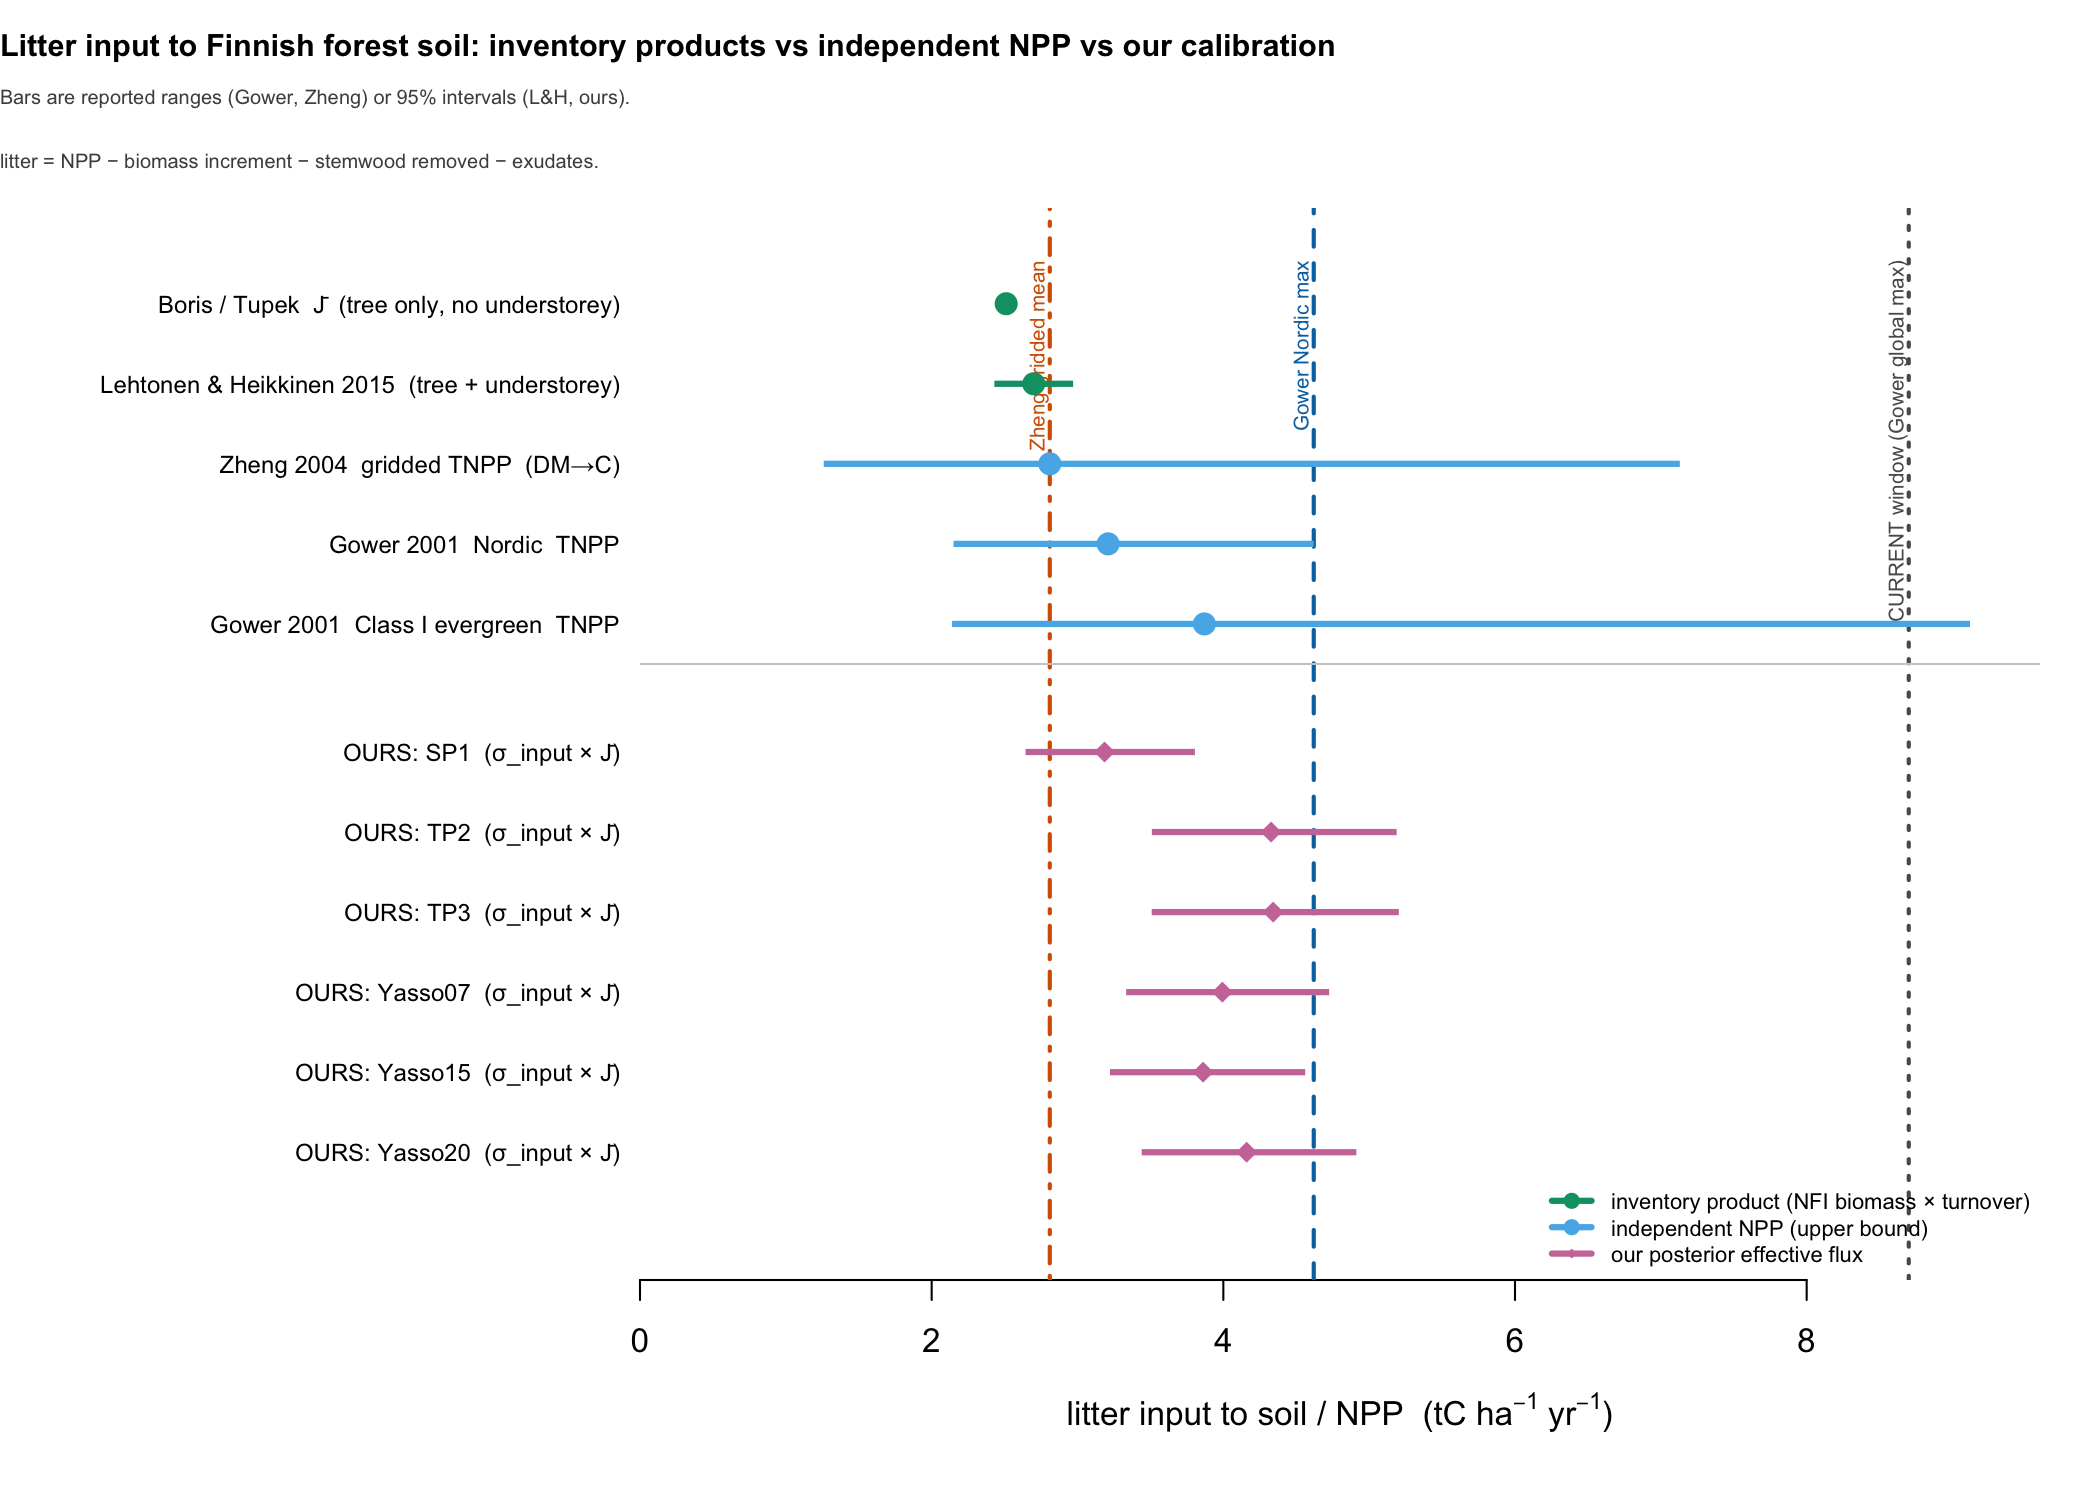
\includegraphics[width=\textwidth,height=0.72\textheight,keepaspectratio]{SX_input_vs_literature}
    \end{column}
    \begin{column}{0.45\textwidth}
      Gap to explain: $0.68$--$1.83$ tC\,ha$^{-1}$\,yr$^{-1}$
      \begin{itemize}
        \item \textbf{Understorey} --- omitted by design; $0.51$--$0.67$ in the NID itself.
        \item \textbf{Mycorrhizal residues} --- not a biomass compartment; plausibly $0.2$--$0.5$.
        \item \textbf{Rhizodeposition} --- standard in cropland accounting (Bolinder 2007); absent from the forest chain.
        \item \textbf{Fine-root lifespan} --- points the \emph{other} way ($\sim$1/3 of the turnover in use).
        \item \textbf{Early succession} --- a timing gap after clear-cut.
      \end{itemize}
      \vspace{0.3em}\textbf{A set that brackets the gap, not a sum that matches it.}
    \end{column}
  \end{columns}
  \note{The most likely reading: the litter model is incomplete, not wrong. Free decomposition rates would have absorbed the missing flux invisibly; anchored rates make it appear. Lehtonen 2016 reached the same conclusion on understorey from the other side. A budget that added up exactly would be MORE suspicious.}
\end{frame}

% =============================================================================
% Q2
% =============================================================================
\section{Result 2 --- does the position on the trade-off matter?}

\begin{frame}{Published vs calibrated, run forward under the same warming}
  \figslide{F15_forward_arms}{0.72}{Neither arm recalibrated; only $\sigma_{\mathrm{input}}$ refitted so both reproduce the observed window. Only \alert{Yasso07} separates ($-2.1$ tC/ha, $[-3.6, -0.8]$, SSP2-4.5). Yasso15/20 do not separate at all.}
  \note{Structural reason: Yasso07 applies ONE climate modifier to every pool, so turnover and temperature sensitivity are the same parameters -- moving along the trade-off moves both. Yasso15/20 have pool-specific modifiers; the humus pool that holds the carbon responds identically in both arms. The result is NOT that 15/20 are right -- it is that they are insensitive to a choice the data cannot settle. Note the main projection has no climate change (recycled 2005-2024 climate, litter at 2024) -- the projected gain is relaxation towards balance.}
\end{frame}

% =============================================================================
% Q3
% =============================================================================
\section{Result 3 --- the plot scale}

\begin{frame}{Between plots, the models describe a gradient the soil does not have}
  \footnotesize
  \begin{columns}[T]
    \begin{column}{0.42\textwidth}
      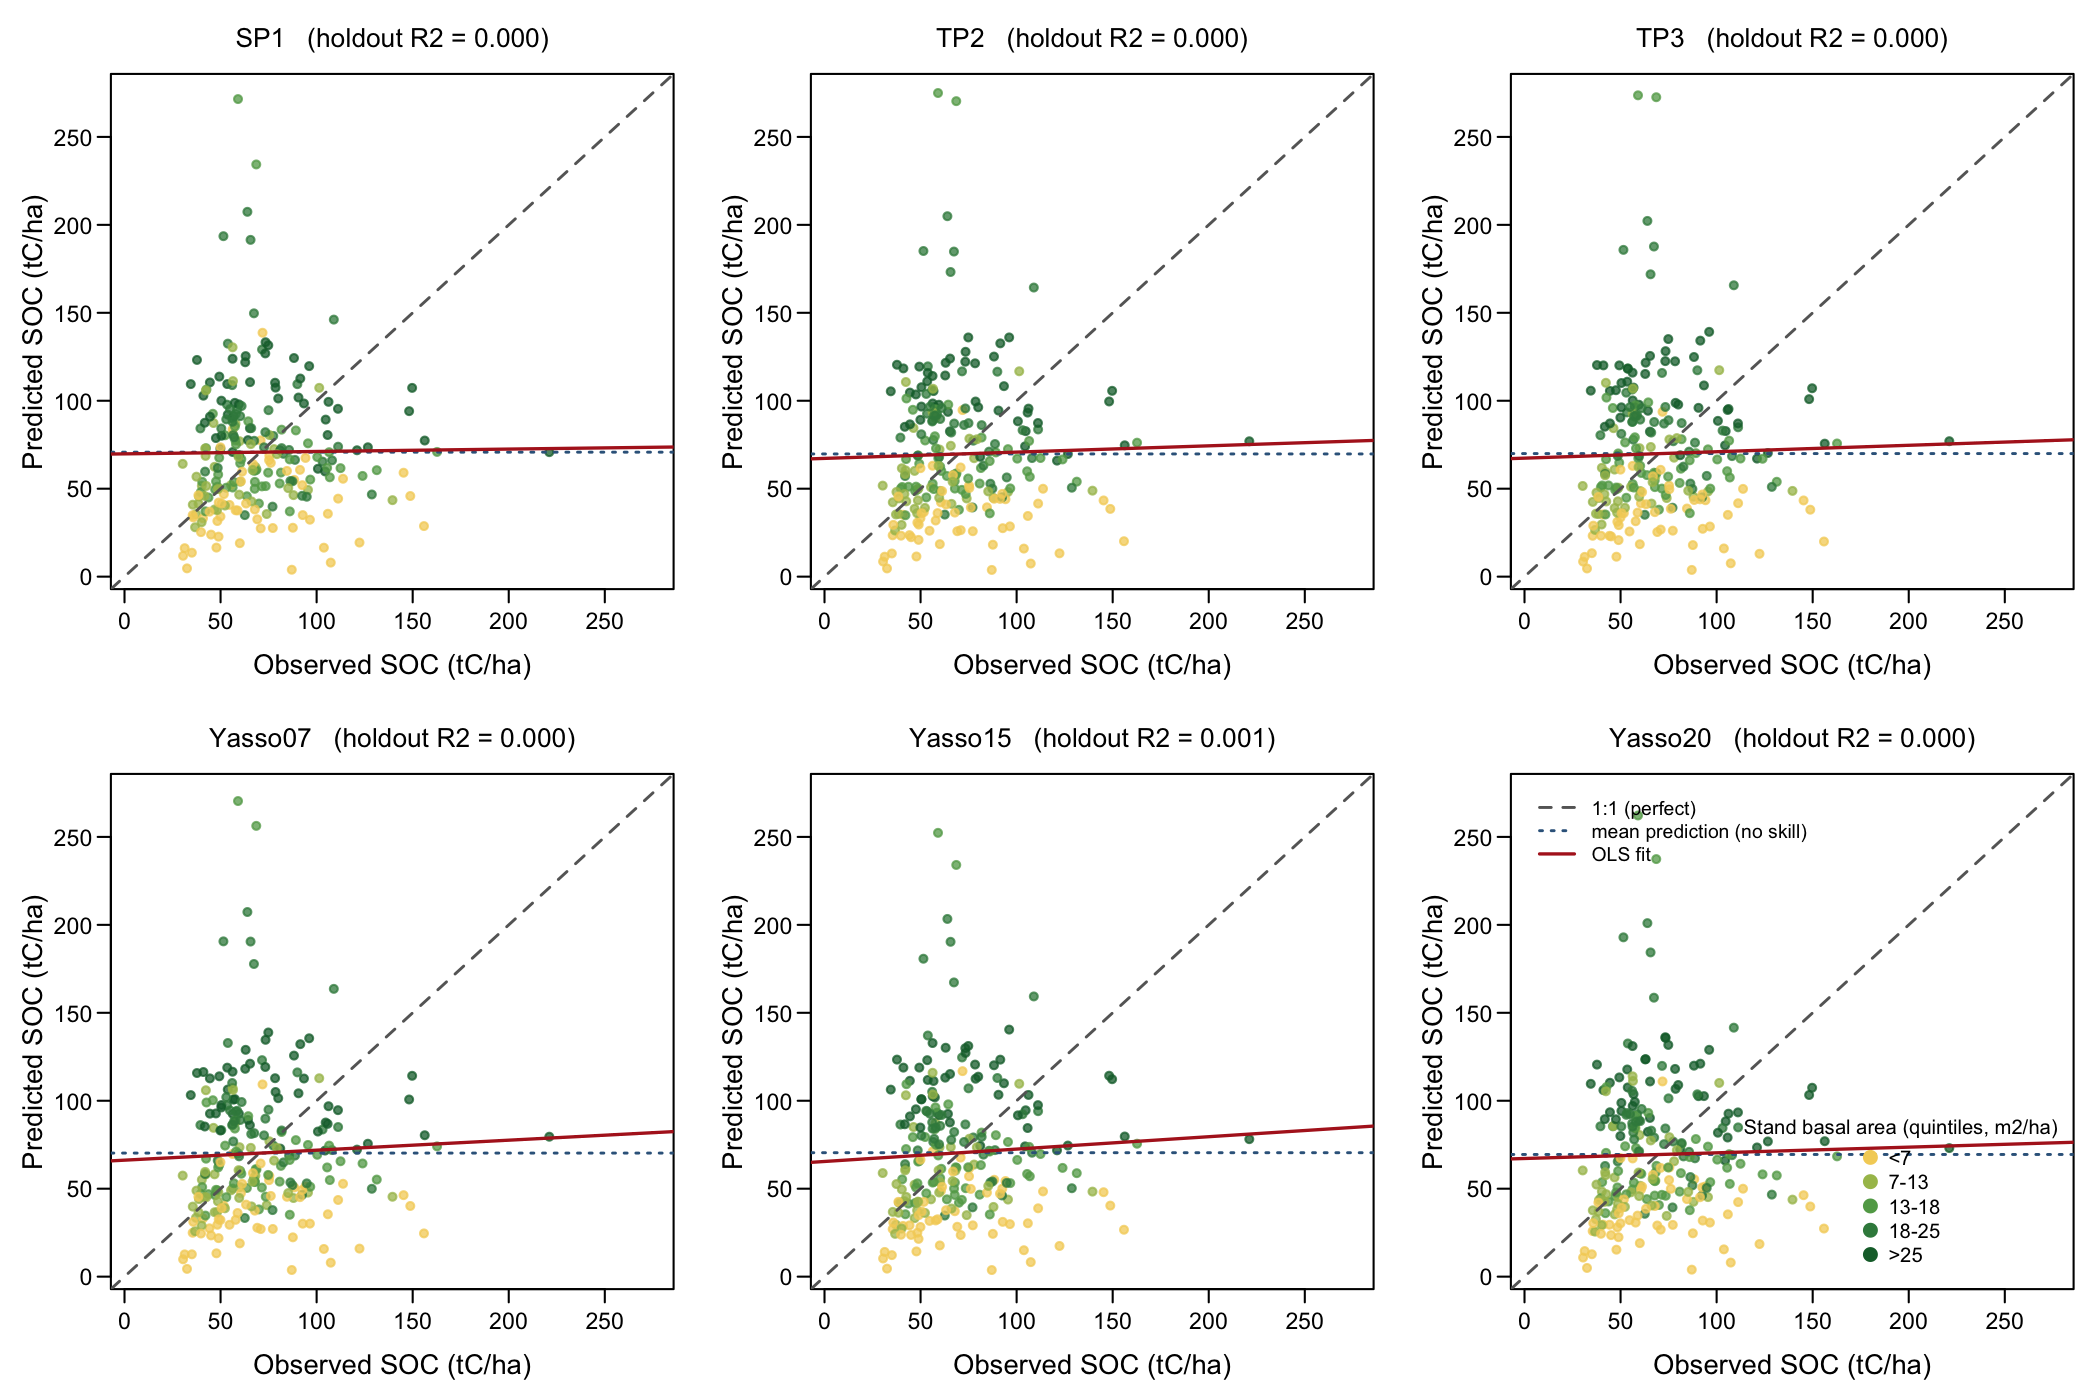
\includegraphics[width=\textwidth,height=0.7\textheight,keepaspectratio]{F6_obs_vs_pred_holdout}
    \end{column}
    \begin{column}{0.58\textwidth}
      \begin{itemize}
        \item Held-out $R^2 = 0$ in all six. What matters is what the models \emph{predict}: stocks ordered by basal area, spread wider than observed.
        \item Slope of $\log$ stock on basal area: models $+0.044$--$0.049$, observed $+0.0044$ (n.s.\ after region and soil).
        \item No model has a basal-area term: the \alert{litter product} rises at $+0.072$ ($\times 18$ across the range) and the models pass it through.
        \item Woody-compartment mismatch tested and \textbf{refuted} (zeroing woody inputs: 6\%; SP1/TP2/TP3 give the same slope with no composition at all).
        \item Plots cut in 1985--95 hold $\sim 40\%$ more C than predicted: the same missing flux, from the other end.
      \end{itemize}
    \end{column}
  \end{columns}
  \note{NEVER say "the models over-apply basal area" -- it reads as a bug and it is not one. Two non-exclusive readings: (1) a plot's stock is not set by its current input -- the paper's argument one level down; (2) an 18-fold input gradient is not credible -- a freshly cut plot does not stop receiving carbon.}
\end{frame}

\begin{frame}{About half of what the models leave behind is recoverable}
  \figslide{F11_rf_heatmap}{0.64}{A random forest on the residuals recovers 44--65\% out of bag, against an observation repeatability of $\sim$0.49. The same variables lead in all six: basal area, development class, coarse fragments. A productivity proxy and a soil property no model has a term for.}
  \note{Recorded and stopped there: choosing the method that would exploit it is not this paper's task. The residual study is a hook whose method is deliberately unnamed.}
\end{frame}

% =============================================================================
% CONCLUSIONS
% =============================================================================
\section{Conclusions}

\begin{frame}{Conclusions}
  \footnotesize
  \begin{enumerate}
    \item A transient, calibrated initial state reproduces a soil C dynamic a steady-state start \alert{cannot} produce: the stocks, the rate, and an accumulation that slows down.
    \item Reproducing it requires \alert{more litter input} (all six) and, graded across the Yassos, faster turnover --- \emph{one} displacement along a trade-off the measurements narrow but do not resolve. It is set by the data, not the prior; the likeliest reading is an incomplete litter input.
    \item The position on the trade-off reaches the \alert{projection} for a model with one climate modifier (Yasso07) and not for models with pool-specific modifiers --- a usable robustness statement for an inventory.
    \item Headroom is real and finite: $+28$ to $+49\%$ to balance at present input (Liski 2006: $+38\%$). Realising it costs decades of sustained input.
    \item Half the plot-scale residual is recoverable from site variables that already exist --- a well-posed next study.
  \end{enumerate}
\end{frame}

\begin{frame}{Where the manuscript stands, and what is still open}
  \footnotesize
  \begin{columns}[T]
    \begin{column}{0.5\textwidth}
      \textbf{Done}
      \begin{itemize}
        \item Draft v1, 36 pp, builds clean; Intro and M\&M through two rounds of comments.
        \item Title chosen; mean \emph{transit} time adopted (Sierra et al.\ 2017).
        \item Literature review, 8 topics; missing-flux budget.
        \item NextGenC deliverable rebuilt on the production run (maps, matrices).
      \end{itemize}
    \end{column}
    \begin{column}{0.5\textwidth}
      \textbf{Open}
      \begin{itemize}
        \item \alert{The equilibrium-init counterfactual has never been run} --- the Introduction's central claim is still theory (design in \texttt{NEXT\_RUN\_equilibrium\_init.md}).
        \item Abstract, Limitations, ``other inventories'' subsection, author block.
        \item Climate citation provisional; prior-criteria table unported.
        \item Data availability: the SOC compilation is not a citable source --- settle with its holders.
        \item F14's Yasso20 dashed line still at the old 19.0 (corrected point 21.9): rebuild.
      \end{itemize}
    \end{column}
  \end{columns}
\end{frame}

% =============================================================================
% BACKUP
% =============================================================================
\appendix
\section{Backup}

\begin{frame}{Backup --- the benchmark trio rides the same ridge, more strongly}
  \figslide{S13_mrt_ridge_benchmark}{0.68}{SP1 / TP2 / TP3, same construction as F14. With the climate modifier included the trio correlates $-0.90$ / $-0.81$ / $-0.81$ --- stronger than any Yasso. The trade-off is a property of the data, not of the five-pool structure.}
\end{frame}

\begin{frame}{Backup --- why the fractions are not identified (and why that is fine)}
  \figslide{F8b_fraction_ridges}{0.68}{Fractions leaving the same pool are near-perfectly anti-correlated: the data fix the net flux out of a pool, not its split. Prior-pinned, ridge-correlated, $<1$ nat --- with clean R-hat.}
\end{frame}

\begin{frame}{Backup --- how tightly is the fit pinned?}
  \figslide{S14_rmse_posterior}{0.68}{RMSE recomputed for every posterior draw. Location = fit; width = how much the posterior disagrees with itself. The cross-run comparison instrument, since log-likelihoods are not comparable across error models.}
\end{frame}

\begin{frame}{Backup --- why only Yasso07 separates in projection}
  \figslide{A1_forward_appendix}{0.57}{Yasso07 applies one $\xi$ to every pool: $\mathrm{MTT} = \mathrm{MTT}_{\mathrm{ref}}/\xi$ exactly, so turnover and temperature sensitivity are the same lever. Yasso15/20 carry $\xi_{AWE}$, $\xi_N$, $\xi_H$; the humus pool that holds the carbon barely moves ($\times 1.04$--$1.06$).}
\end{frame}

\begin{frame}{Backup --- the observed rate: what it rests on}
  \footnotesize
  \begin{columns}[T]
    \begin{column}{0.42\textwidth}
      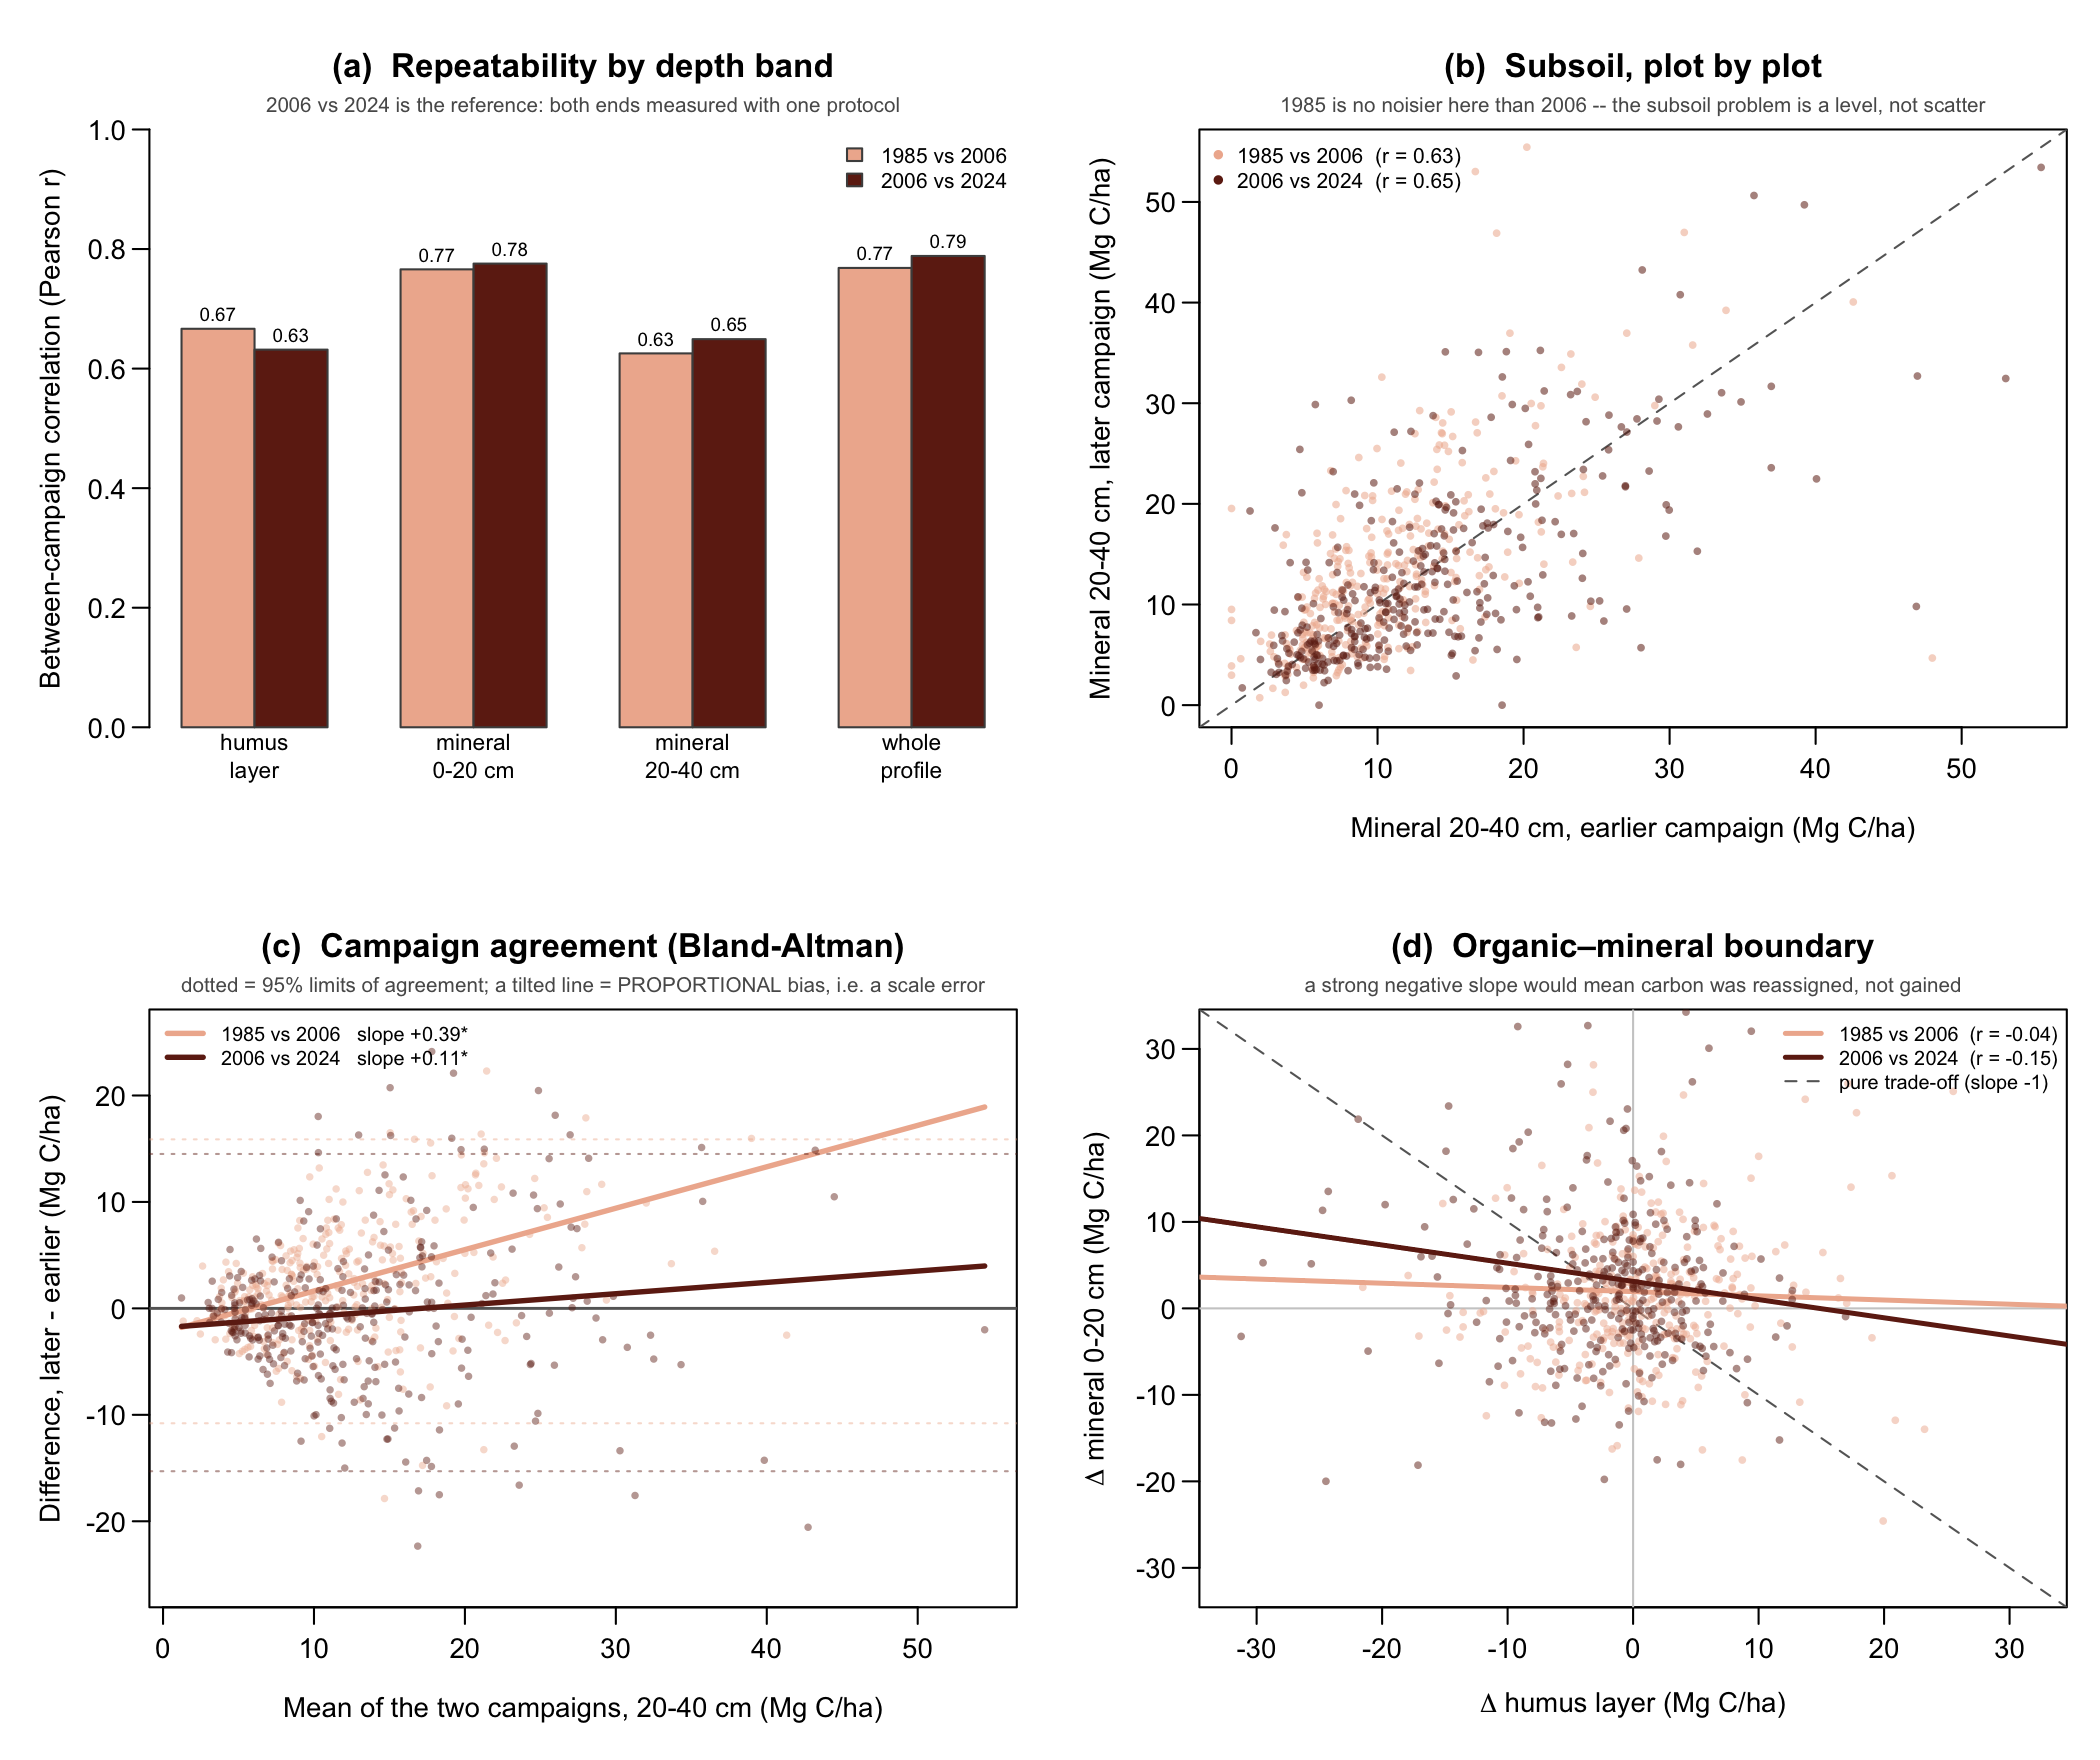
\includegraphics[width=\textwidth,height=0.7\textheight,keepaspectratio]{S10_soc_campaign_reliability}
    \end{column}
    \begin{column}{0.58\textwidth}
      \begin{itemize}
        \item Basis (decided): balanced set $n=310$, unweighted, whole profile, true years. Worth $1.8\times$ on the 2006--2024 rate ($+0.117$ vs $+0.209$ pairwise).
        \item 1985 organic layer was OFH only; the missing litter+moss layer ($3.4$--$4.3$ Mg C/ha) was 89\% of the apparent 1985$\to$2006 organic gain. Each plot's own 2006 LM added.
        \item ``1985'' is 1986--1995 (19.5\% of plots in 1995): interval to 2024 is $35.1$ yr, not 39.
        \item Full-window rate survives a 9\% shared offset; the last-interval rate dissolves at 2\%.
      \end{itemize}
    \end{column}
  \end{columns}
\end{frame}

\begin{frame}{Backup --- the error model, and why the total is above the measured spread}
  \footnotesize
  \begin{columns}[T]
    \begin{column}{0.5\textwidth}
      \small
      \scriptsize
      \begin{tabular}{lcc}
        \toprule
        term & SD & measured on \\
        \midrule
        region $u^R$ & 0.117 & 8 latitude bands \\
        plot $u^P$ & 0.396 & same-plot pair covariance \\
        campaign $u^C$ & 0.060 / 0.030 & prescribed \\
        residual $e$ & 0.685 & remainder \\
        \midrule
        total & \textbf{0.800} & fixed \\
        \bottomrule
      \end{tabular}
    \end{column}
    \begin{column}{0.5\textwidth}
      \small
      \begin{itemize}
        \item 1205 plot-years are not independent: plot ICC $0.57$--$0.71$ ($n_{\mathrm{eff}} \approx 630$); latitude-band means vary $5$--$6\times$ more than iid allows.
        \item Uniform $\sigma$ inflation broadens every direction by $\sqrt{k}$; only correlated structure broadens the \emph{level} direction at fixed total variance.
        \item Design rule: residuals may \emph{check} a design value, never set one.
        \item $\tau = 0$ reproduces the independent log-normal likelihood exactly (unit-tested).
      \end{itemize}
    \end{column}
  \end{columns}
\end{frame}

\begin{frame}{Backup --- the 1917 state the models imply}
  \scriptsize
  \begin{tabular}{lcccccc}
    \toprule
    & $\sigma_{\mathrm{init}}$ & $J_{1917}$ & $J_{1985}$ & $C_{1917}$ & $C_{1985}$ & pre-run rate \\
    \midrule
    SP1     & 0.63 & 2.32 & 3.68 & 39.5 & 49.1 & $+0.148$ \\
    TP2     & 0.45 & 1.90 & 4.36 & 32.8 & 44.8 & $+0.181$ \\
    TP3     & 0.43 & 1.73 & 4.14 & 32.6 & 44.6 & $+0.177$ \\
    Yasso07 & 0.32 & 1.50 & 4.67 & 30.8 & 45.2 & $+0.217$ \\
    Yasso15 & 0.29 & 1.27 & 4.22 & 30.1 & 47.0 & $+0.242$ \\
    Yasso20 & 0.33 & 1.47 & 4.56 & 31.3 & 47.9 & $+0.235$ \\
    \bottomrule
  \end{tabular}
  \vspace{0.6em}

  Run 20260817 (the previous run; the current one moved $\sigma_{\mathrm{init}}$ up to 0.49--0.84). Fluxes in tC\,ha$^{-1}$\,yr$^{-1}$, stocks in tC/ha. The pre-run rate is \emph{below} the observed $+0.259$ in all six. The 1917 stock (30--40 tC/ha) is \textbf{reported, not constrained}; the growing-stock bound on $\sigma_{\mathrm{init}}$ was retired because judging our start by an equilibrium benchmark re-imports the convention the paper argues against.
\end{frame}

\begin{frame}{Backup --- equilibrium headroom}
  \begin{itemize}
    \item Hold litter at its present level and let each calibrated model run to its own balance: the soil sits \alert{$28$--$49\%$ below} that balance in five of six models (SP1: $+5\%$).
    \item Liski et al.\ 2006, from an assumed 1922 steady state and the same forward simulation: $+38\%$ ``centuries later''.
    \item Two routes, one answer on \emph{how far} the soil is from balance --- and both say the room is finite.
    \item The main projection has \textbf{no climate change}: 2005--2024 climate recycled, litter frozen at 2024. The projected gain is relaxation towards balance, not a warming response.
  \end{itemize}
\end{frame}

\begin{frame}{Backup --- the deliverable: gridded SOC and its uncertainty}
  \begin{columns}[T]
    \begin{column}{0.32\textwidth}\centering
      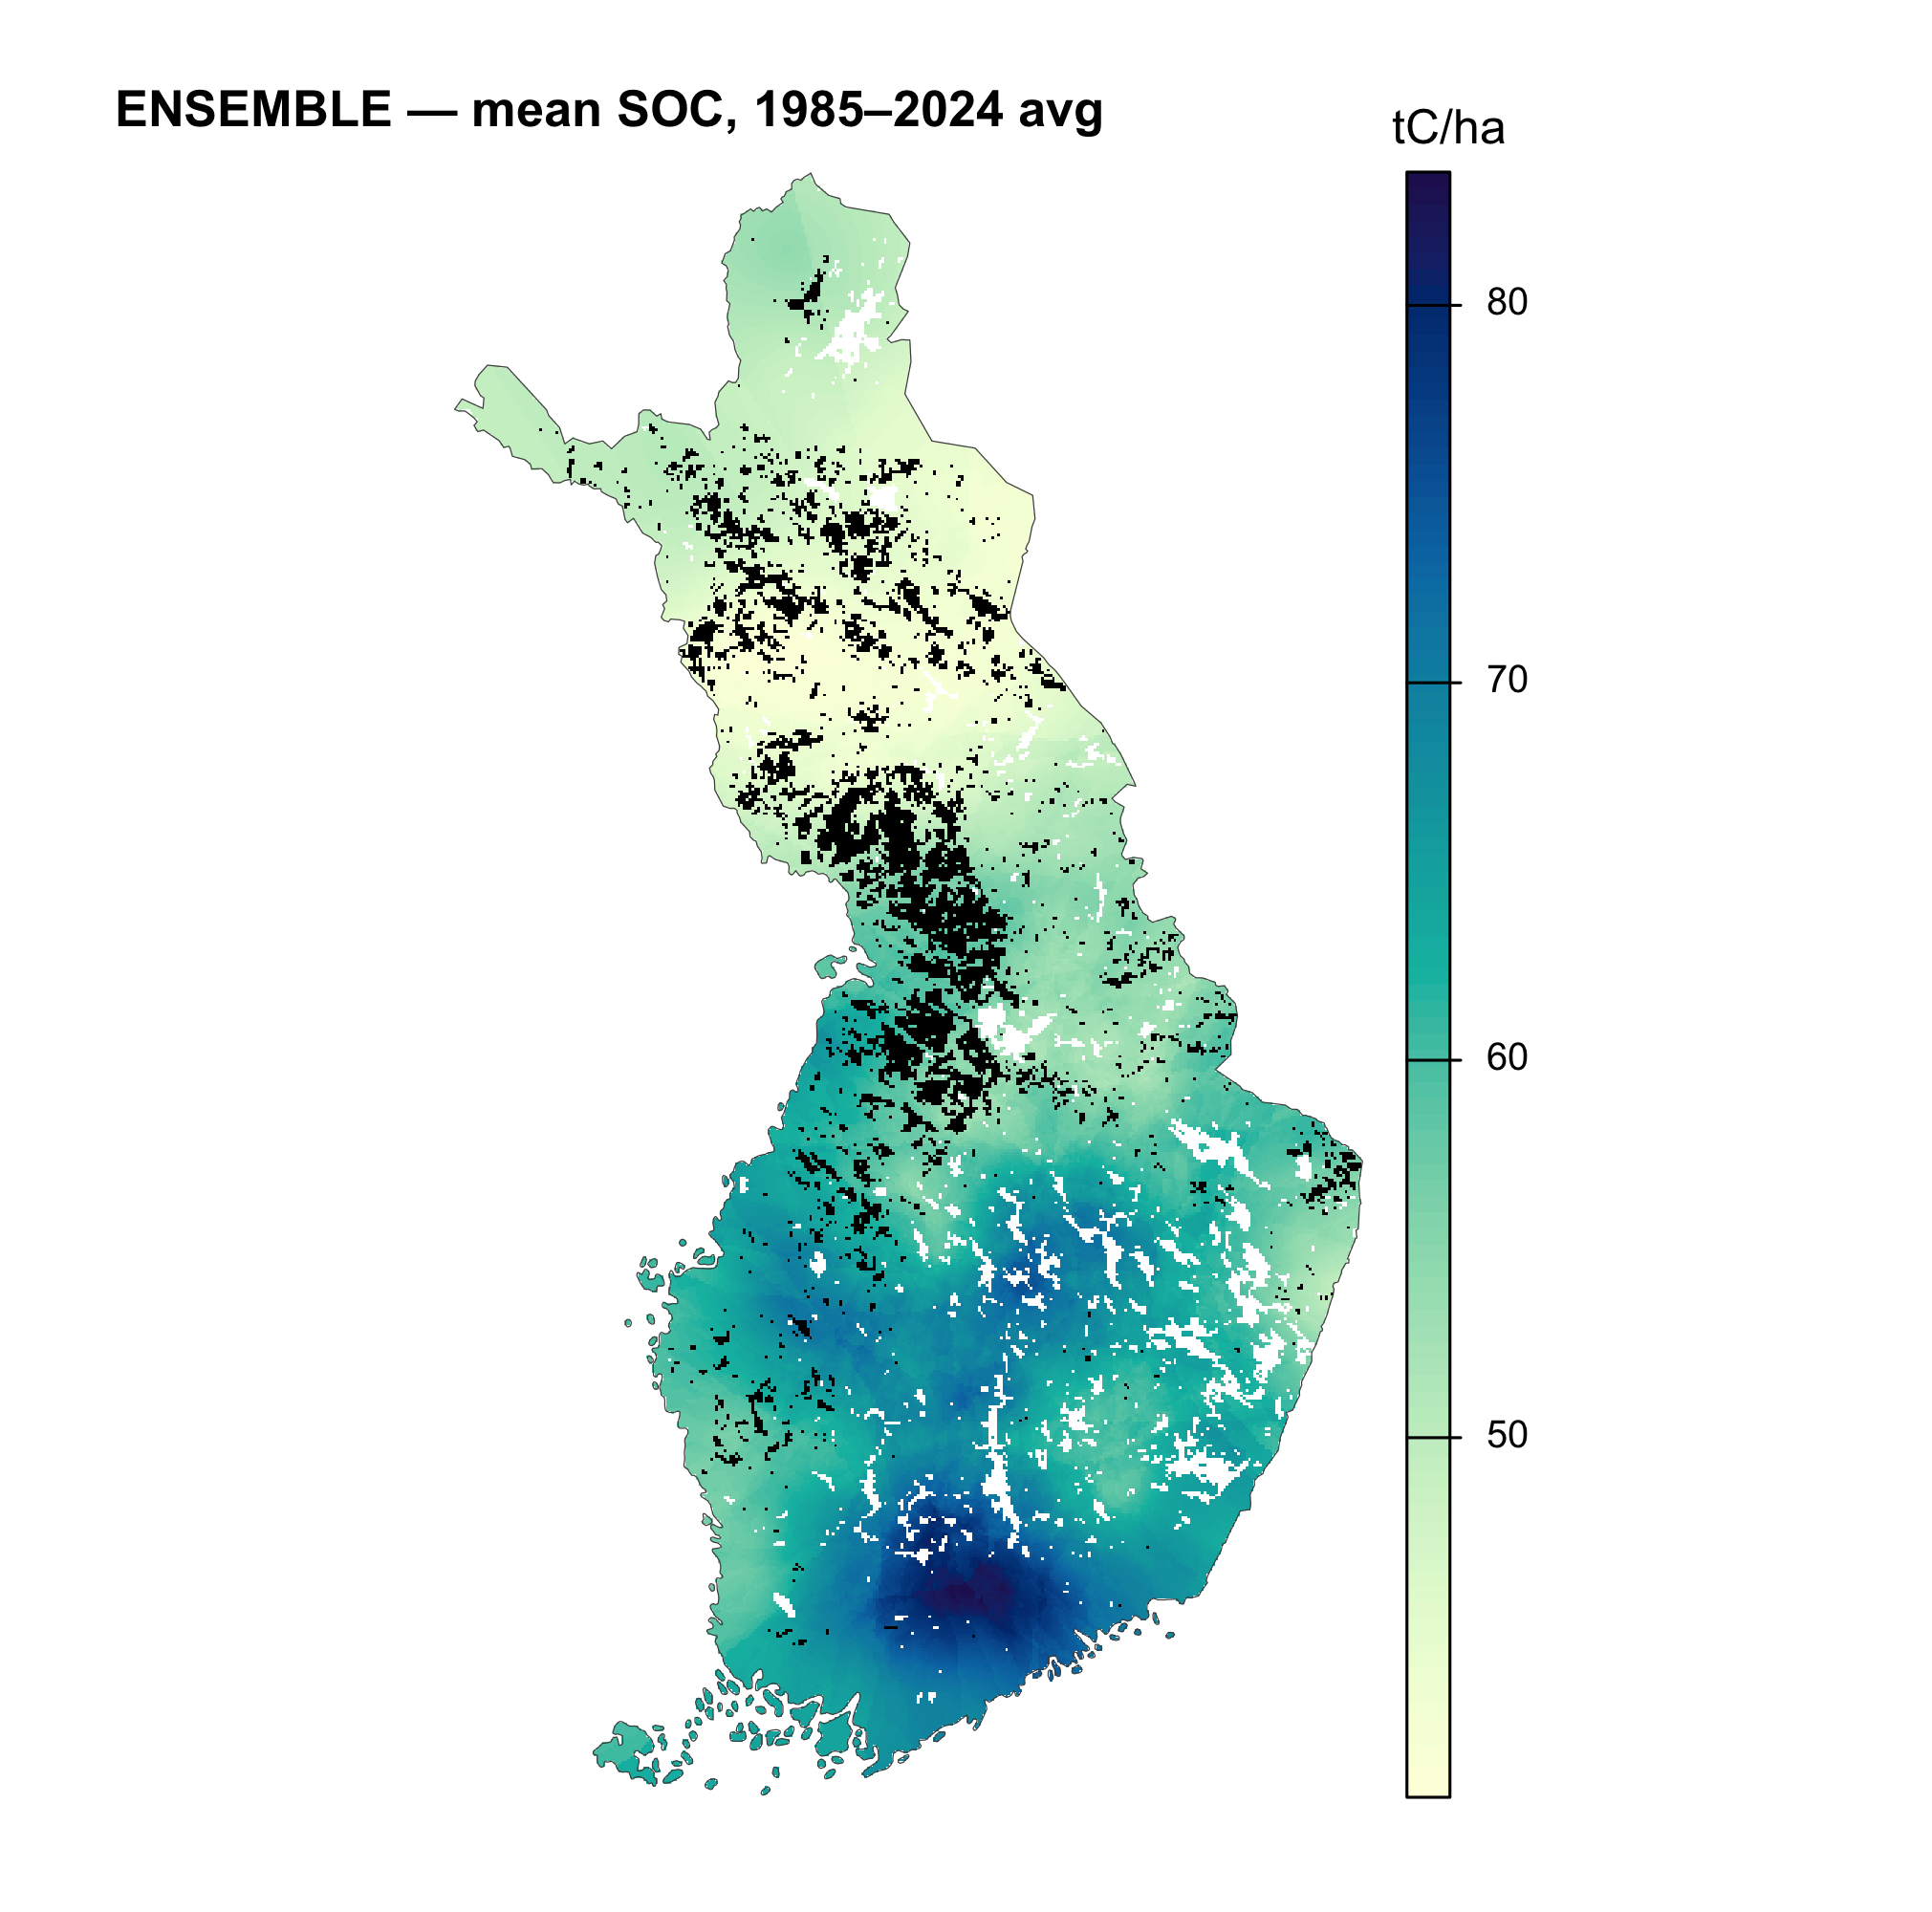
\includegraphics[height=0.58\textheight,width=\textwidth,keepaspectratio]{ENSEMBLE_SOC_mean}\\ {\scriptsize ensemble mean}
    \end{column}
    \begin{column}{0.32\textwidth}\centering
      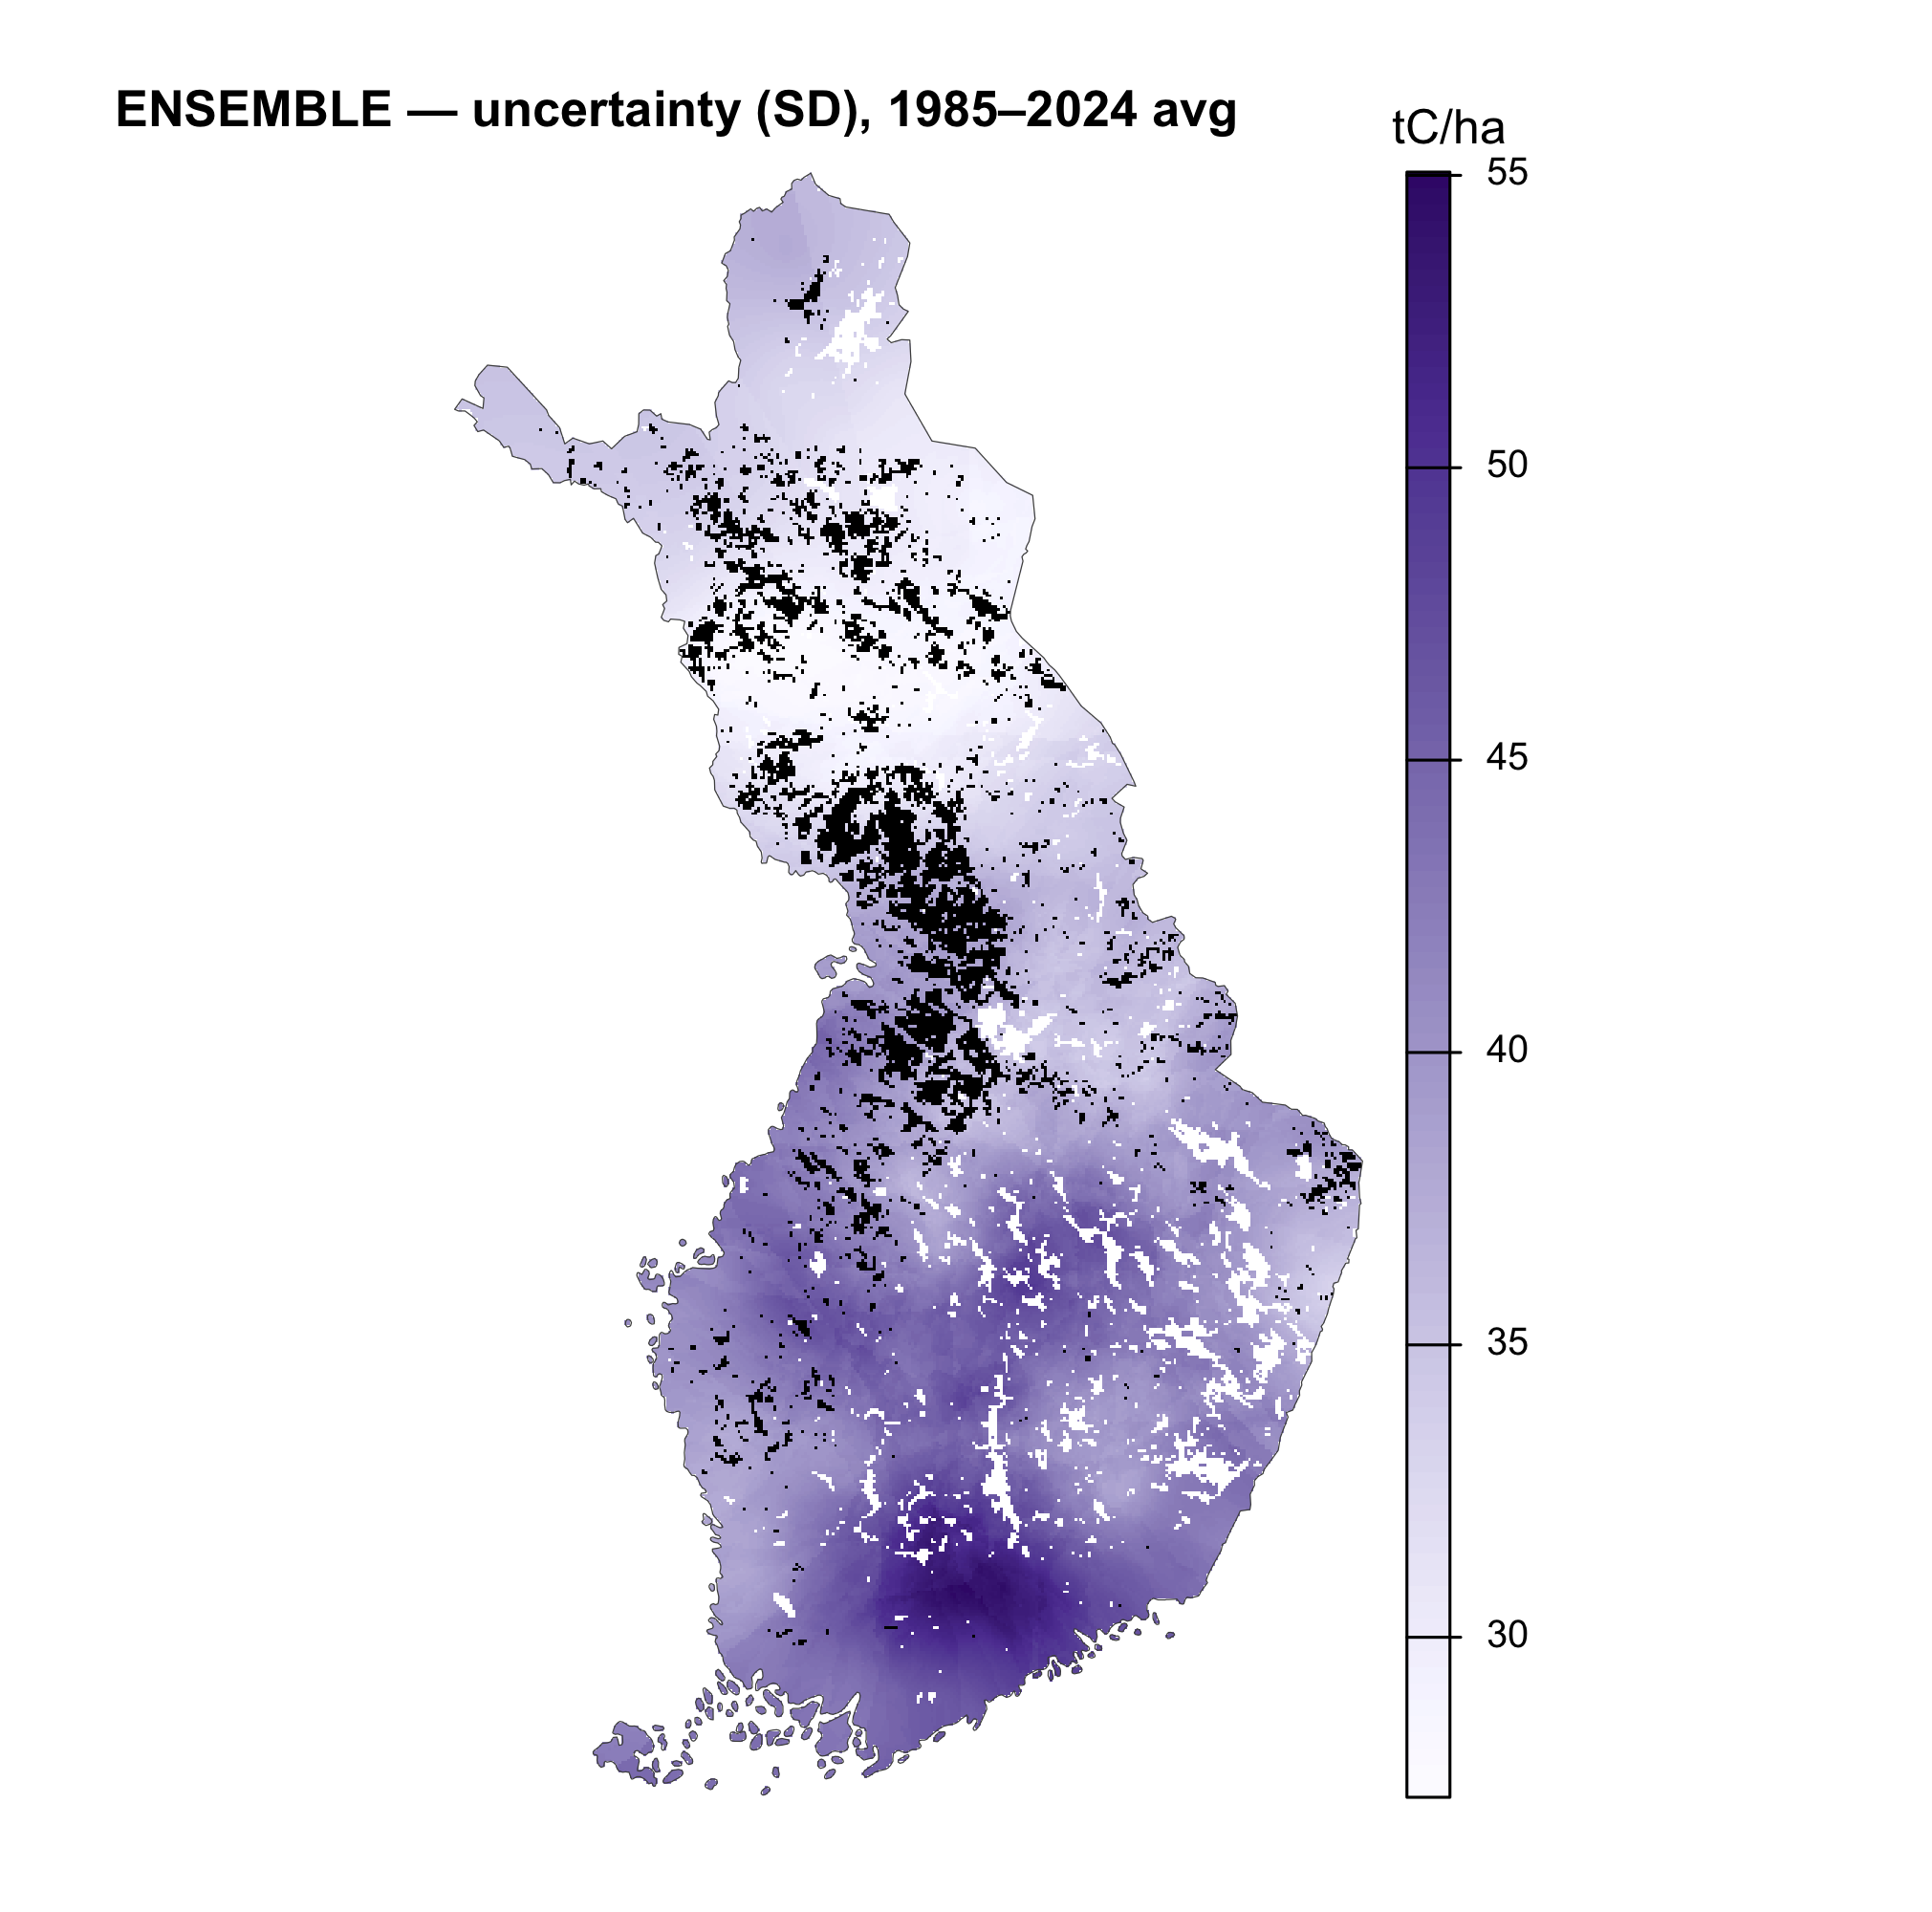
\includegraphics[height=0.58\textheight,width=\textwidth,keepaspectratio]{ENSEMBLE_SOC_sd}\\ {\scriptsize ensemble SD}
    \end{column}
    \begin{column}{0.32\textwidth}\centering
      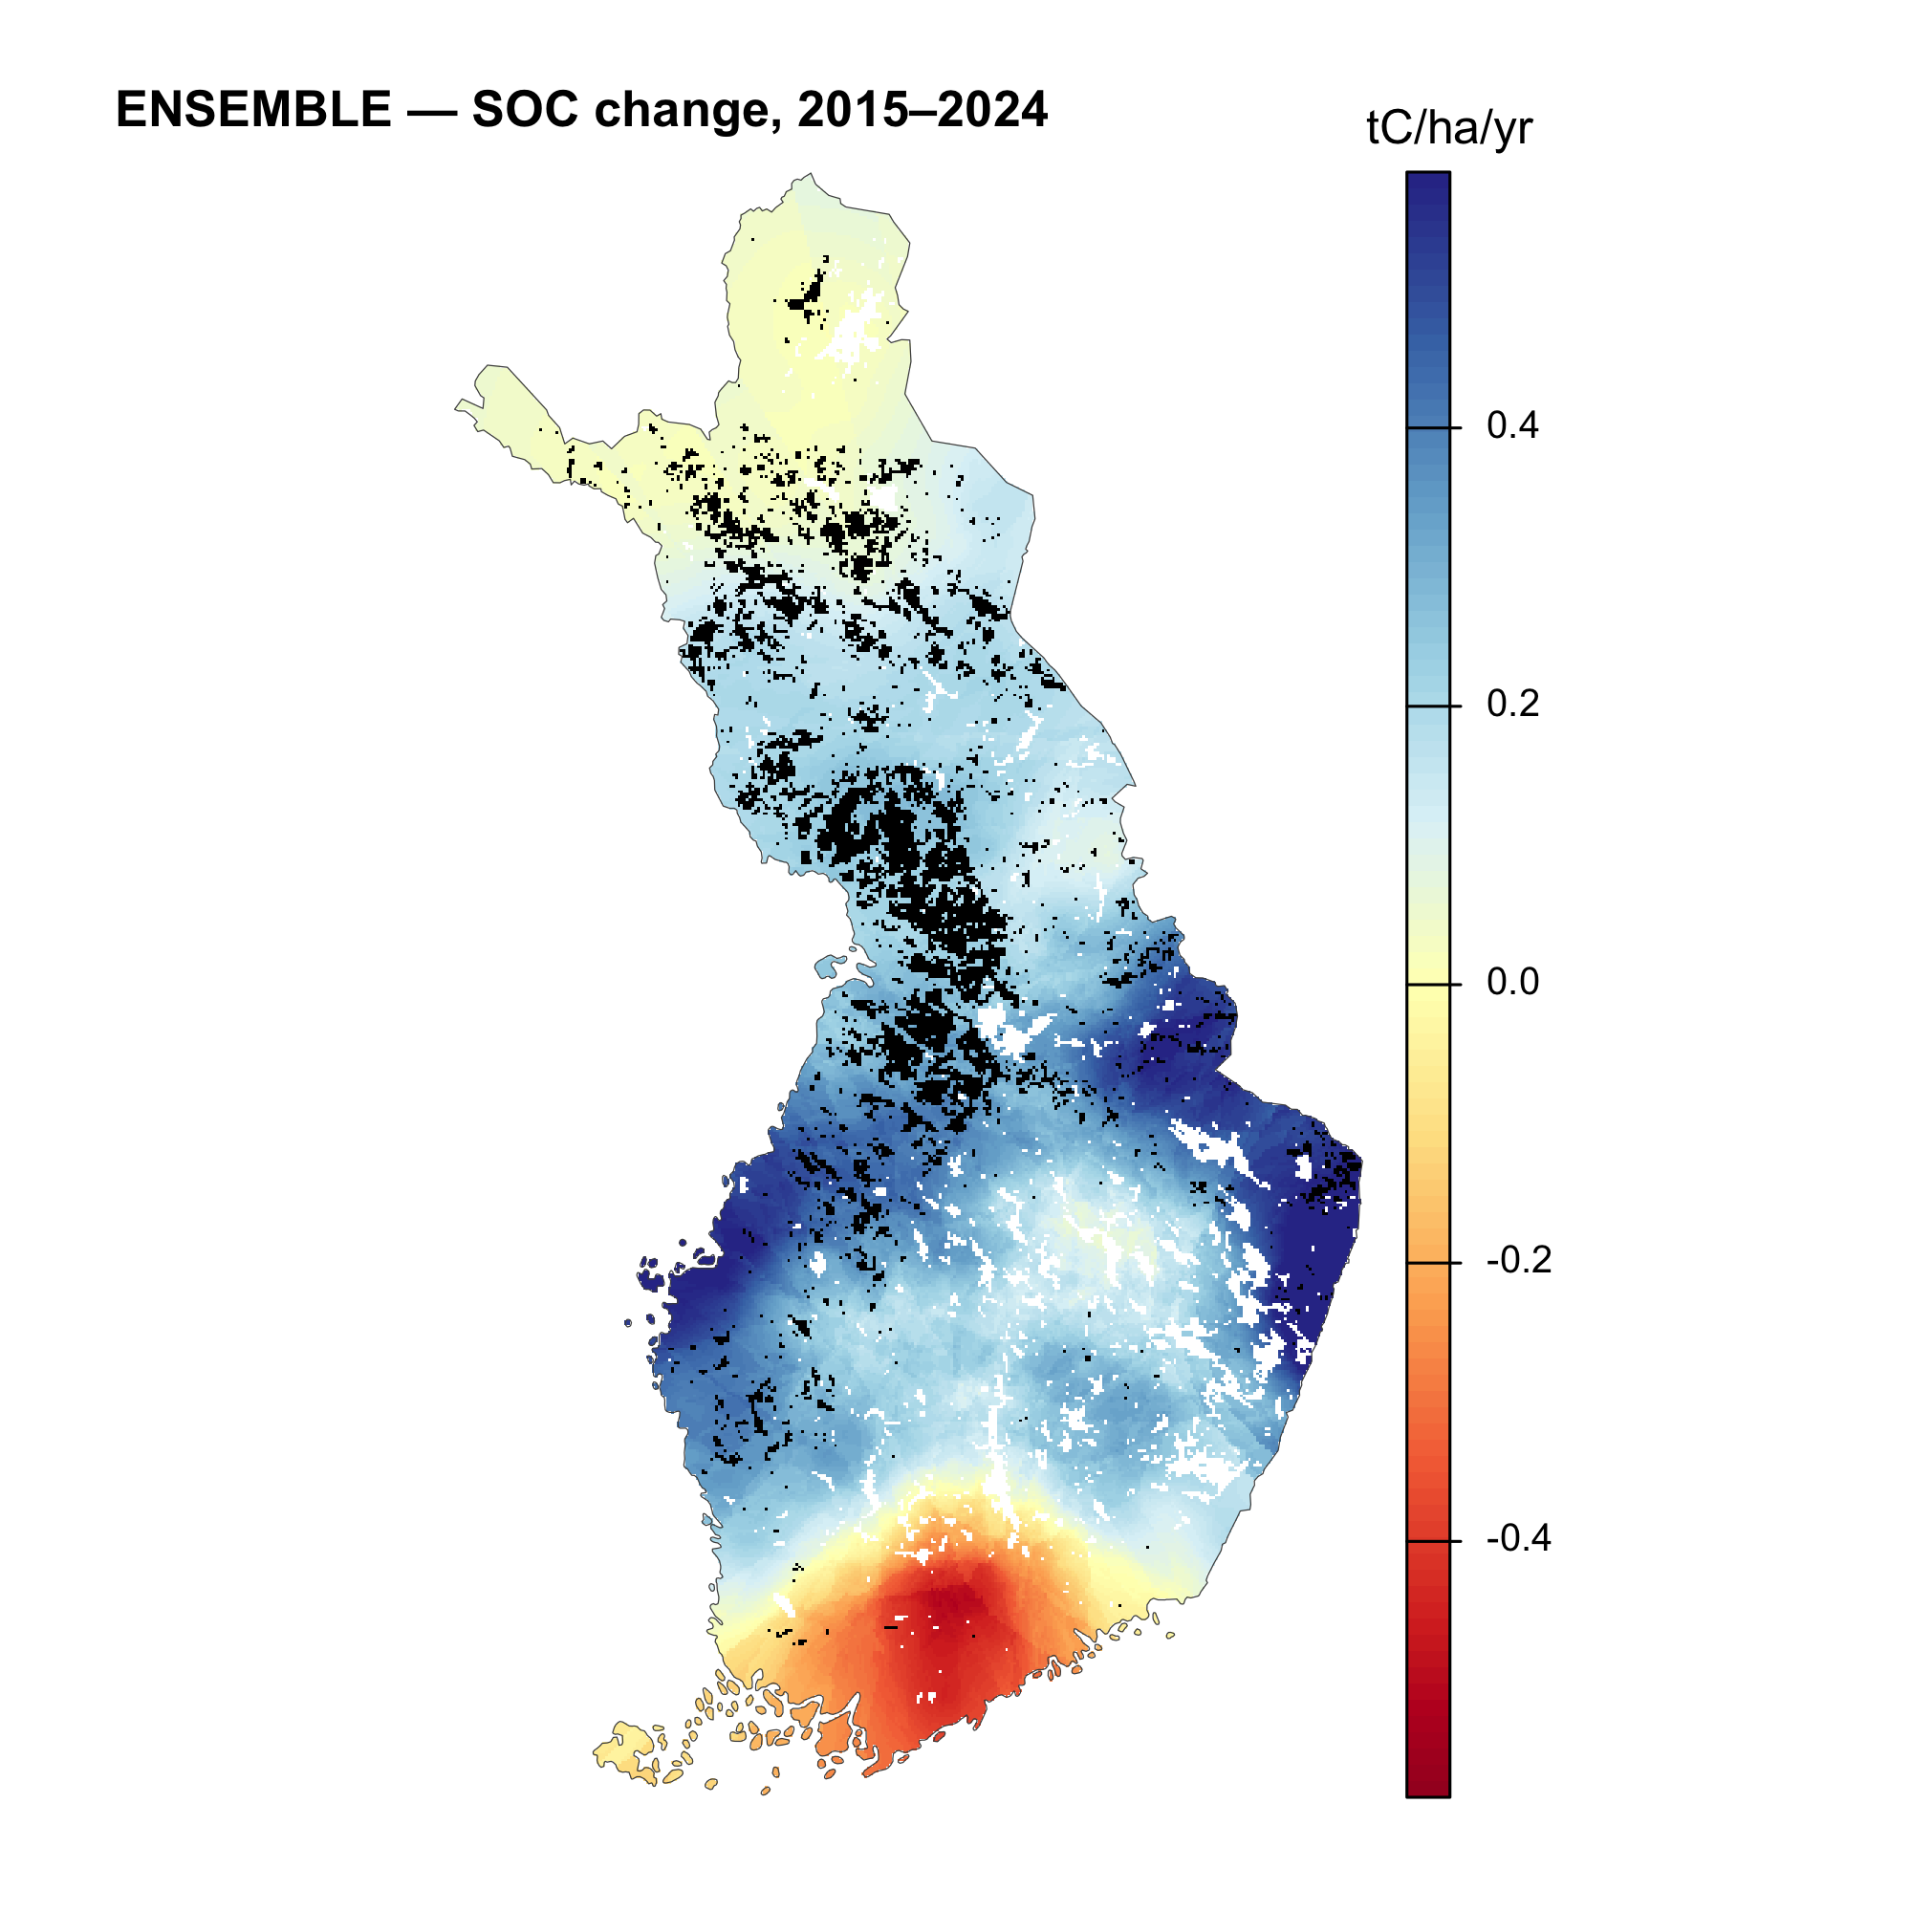
\includegraphics[height=0.58\textheight,width=\textwidth,keepaspectratio]{ENSEMBLE_SOC_delta10yr}\\ {\scriptsize decadal change}
    \end{column}
  \end{columns}
  \takeaway{Six-model ensemble, kriged to 2 km, historical 1985--2024 only (no projection). NextGenC / Zenodo deposit, CC-BY-4.0. A bonus product, not a conclusion.}
\end{frame}

\begin{frame}{Backup --- convergence}
  \figslide{R1_convergence}{0.72}{All parameters R-hat $\le 1.008$, ESS $\ge 1450$, numerically impossible proposals $\sim 0\%$ in all six models (production run 20260831).}
\end{frame}

\end{document}
